% Options for packages loaded elsewhere
\PassOptionsToPackage{unicode}{hyperref}
\PassOptionsToPackage{hyphens}{url}
%
\documentclass[
]{book}
\usepackage{lmodern}
\usepackage{amsmath}
\usepackage{ifxetex,ifluatex}
\ifnum 0\ifxetex 1\fi\ifluatex 1\fi=0 % if pdftex
  \usepackage[T1]{fontenc}
  \usepackage[utf8]{inputenc}
  \usepackage{textcomp} % provide euro and other symbols
  \usepackage{amssymb}
\else % if luatex or xetex
  \usepackage{unicode-math}
  \defaultfontfeatures{Scale=MatchLowercase}
  \defaultfontfeatures[\rmfamily]{Ligatures=TeX,Scale=1}
\fi
% Use upquote if available, for straight quotes in verbatim environments
\IfFileExists{upquote.sty}{\usepackage{upquote}}{}
\IfFileExists{microtype.sty}{% use microtype if available
  \usepackage[]{microtype}
  \UseMicrotypeSet[protrusion]{basicmath} % disable protrusion for tt fonts
}{}
\makeatletter
\@ifundefined{KOMAClassName}{% if non-KOMA class
  \IfFileExists{parskip.sty}{%
    \usepackage{parskip}
  }{% else
    \setlength{\parindent}{0pt}
    \setlength{\parskip}{6pt plus 2pt minus 1pt}}
}{% if KOMA class
  \KOMAoptions{parskip=half}}
\makeatother
\usepackage{xcolor}
\IfFileExists{xurl.sty}{\usepackage{xurl}}{} % add URL line breaks if available
\IfFileExists{bookmark.sty}{\usepackage{bookmark}}{\usepackage{hyperref}}
\hypersetup{
  pdftitle={Academy for Dummies},
  pdfauthor={Team Algoritma},
  hidelinks,
  pdfcreator={LaTeX via pandoc}}
\urlstyle{same} % disable monospaced font for URLs
\usepackage{color}
\usepackage{fancyvrb}
\newcommand{\VerbBar}{|}
\newcommand{\VERB}{\Verb[commandchars=\\\{\}]}
\DefineVerbatimEnvironment{Highlighting}{Verbatim}{commandchars=\\\{\}}
% Add ',fontsize=\small' for more characters per line
\usepackage{framed}
\definecolor{shadecolor}{RGB}{248,248,248}
\newenvironment{Shaded}{\begin{snugshade}}{\end{snugshade}}
\newcommand{\AlertTok}[1]{\textcolor[rgb]{0.94,0.16,0.16}{#1}}
\newcommand{\AnnotationTok}[1]{\textcolor[rgb]{0.56,0.35,0.01}{\textbf{\textit{#1}}}}
\newcommand{\AttributeTok}[1]{\textcolor[rgb]{0.77,0.63,0.00}{#1}}
\newcommand{\BaseNTok}[1]{\textcolor[rgb]{0.00,0.00,0.81}{#1}}
\newcommand{\BuiltInTok}[1]{#1}
\newcommand{\CharTok}[1]{\textcolor[rgb]{0.31,0.60,0.02}{#1}}
\newcommand{\CommentTok}[1]{\textcolor[rgb]{0.56,0.35,0.01}{\textit{#1}}}
\newcommand{\CommentVarTok}[1]{\textcolor[rgb]{0.56,0.35,0.01}{\textbf{\textit{#1}}}}
\newcommand{\ConstantTok}[1]{\textcolor[rgb]{0.00,0.00,0.00}{#1}}
\newcommand{\ControlFlowTok}[1]{\textcolor[rgb]{0.13,0.29,0.53}{\textbf{#1}}}
\newcommand{\DataTypeTok}[1]{\textcolor[rgb]{0.13,0.29,0.53}{#1}}
\newcommand{\DecValTok}[1]{\textcolor[rgb]{0.00,0.00,0.81}{#1}}
\newcommand{\DocumentationTok}[1]{\textcolor[rgb]{0.56,0.35,0.01}{\textbf{\textit{#1}}}}
\newcommand{\ErrorTok}[1]{\textcolor[rgb]{0.64,0.00,0.00}{\textbf{#1}}}
\newcommand{\ExtensionTok}[1]{#1}
\newcommand{\FloatTok}[1]{\textcolor[rgb]{0.00,0.00,0.81}{#1}}
\newcommand{\FunctionTok}[1]{\textcolor[rgb]{0.00,0.00,0.00}{#1}}
\newcommand{\ImportTok}[1]{#1}
\newcommand{\InformationTok}[1]{\textcolor[rgb]{0.56,0.35,0.01}{\textbf{\textit{#1}}}}
\newcommand{\KeywordTok}[1]{\textcolor[rgb]{0.13,0.29,0.53}{\textbf{#1}}}
\newcommand{\NormalTok}[1]{#1}
\newcommand{\OperatorTok}[1]{\textcolor[rgb]{0.81,0.36,0.00}{\textbf{#1}}}
\newcommand{\OtherTok}[1]{\textcolor[rgb]{0.56,0.35,0.01}{#1}}
\newcommand{\PreprocessorTok}[1]{\textcolor[rgb]{0.56,0.35,0.01}{\textit{#1}}}
\newcommand{\RegionMarkerTok}[1]{#1}
\newcommand{\SpecialCharTok}[1]{\textcolor[rgb]{0.00,0.00,0.00}{#1}}
\newcommand{\SpecialStringTok}[1]{\textcolor[rgb]{0.31,0.60,0.02}{#1}}
\newcommand{\StringTok}[1]{\textcolor[rgb]{0.31,0.60,0.02}{#1}}
\newcommand{\VariableTok}[1]{\textcolor[rgb]{0.00,0.00,0.00}{#1}}
\newcommand{\VerbatimStringTok}[1]{\textcolor[rgb]{0.31,0.60,0.02}{#1}}
\newcommand{\WarningTok}[1]{\textcolor[rgb]{0.56,0.35,0.01}{\textbf{\textit{#1}}}}
\usepackage{longtable,booktabs}
\usepackage{calc} % for calculating minipage widths
% Correct order of tables after \paragraph or \subparagraph
\usepackage{etoolbox}
\makeatletter
\patchcmd\longtable{\par}{\if@noskipsec\mbox{}\fi\par}{}{}
\makeatother
% Allow footnotes in longtable head/foot
\IfFileExists{footnotehyper.sty}{\usepackage{footnotehyper}}{\usepackage{footnote}}
\makesavenoteenv{longtable}
\usepackage{graphicx}
\makeatletter
\def\maxwidth{\ifdim\Gin@nat@width>\linewidth\linewidth\else\Gin@nat@width\fi}
\def\maxheight{\ifdim\Gin@nat@height>\textheight\textheight\else\Gin@nat@height\fi}
\makeatother
% Scale images if necessary, so that they will not overflow the page
% margins by default, and it is still possible to overwrite the defaults
% using explicit options in \includegraphics[width, height, ...]{}
\setkeys{Gin}{width=\maxwidth,height=\maxheight,keepaspectratio}
% Set default figure placement to htbp
\makeatletter
\def\fps@figure{htbp}
\makeatother
\setlength{\emergencystretch}{3em} % prevent overfull lines
\providecommand{\tightlist}{%
  \setlength{\itemsep}{0pt}\setlength{\parskip}{0pt}}
\setcounter{secnumdepth}{5}
\usepackage{booktabs}
\ifluatex
  \usepackage{selnolig}  % disable illegal ligatures
\fi
\usepackage[]{natbib}
\bibliographystyle{apalike}

\title{Academy for Dummies}
\author{Team Algoritma}
\date{31, Maret 2021}

\begin{document}
\maketitle

{
\setcounter{tocdepth}{1}
\tableofcontents
}
\hypertarget{introduction}{%
\chapter{Introduction}\label{introduction}}

\textbf{Academy for Dummies (A4D)} ditulis oleh tim Algoritma untuk panduan seluruh tim yang bertugas dan berhubungan dengan kegiatan dalam Algoritma Academy. Mohon untuk mempelajari beberapa hal berikut sebelum bertugas.

\hypertarget{fasilitas-student}{%
\chapter{Fasilitas Student}\label{fasilitas-student}}

Setiap student memiliki beberapa administrasi yang perlu diketahui dan diikuti selama mengikuti kelas Algoritma Academy.

\hypertarget{pengajuan-mentoring}{%
\section{Pengajuan Mentoring}\label{pengajuan-mentoring}}

Mentoring merupakan salah satu fasilitas yang diterima oleh student Algoritma berupa sesi 101 dengan mentor Algoritma untuk menanyakan hal-hal yang belum dipahami dan ingin dipelajari lebih lanjut. Berikut ini beberapa peraturan yang berhubungan dengan mentoring:

\begin{enumerate}
\def\labelenumi{\arabic{enumi}.}
\tightlist
\item
  Mentoring dilaksanakan \textbf{1x/minggu} dengan durasi 1 jam pada hari kerja Senin-Jumat pukul 10:00-18:00.
\item
  Pengajuan mentoring terpusat melalui email \textbf{\href{mailto:mentor@algorit.ma}{\nolinkurl{mentor@algorit.ma}}}.
\item
  Permintaan mentoring dilakukan \textbf{maksimal H-1 sebelum hari mentoring} yang diinginkan pada hari Senin-Jumat pukul 10:00-18:00 WIB, dengan template permintaan mentoring sebagai berikut:
\end{enumerate}

\begin{verbatim}
Berikan subject email : ALGORITMA MENTORING SESSION
Nama : ___________
Kelas : ___________ (nama batch day / night)
Materi mentoring : ___________
Tanggal, Jam mentoring : ___________
\end{verbatim}

\begin{enumerate}
\def\labelenumi{\arabic{enumi}.}
\setcounter{enumi}{3}
\tightlist
\item
  Permintaan mentoring yang diajukan melewati jam kerja akan dibalas pada hari berikutnya dan pelaksanaan mentoring tidak dapat dilakukan pada hari yang sama.
\item
  Pengajuan mentoring yang tidak sesuai dengan template yang ada maka akan dikembalikan kepada student kembali hingga informasi pada template mentoring sudah terpenuhi. Apabila informasi pada template telah terpenuhi, mentoring baru akan diproses.
\item
  Apabila terdapat lebih dari satu permintaan mentoring dengan waktu serta materi yang sama, maka admin dapat menawarkan untuk dilakukan secara bersamaan dengan mentor yang sama.
\item
  Student tidak diperkenankan untuk memilih mentor untuk membantunya selama mentoring.
\item
  Apabila course dalam batch academy telah selesai, student diberikan fasilitas untuk mengajukan mentoring \textbf{hingga 4 minggu} (hari kerja dan hari libur) setelah capstone project sesuai dengan spesialisasi yang diambil.
\end{enumerate}

\hypertarget{pengajuan-pertanyaan}{%
\section{Pengajuan Pertanyaan}\label{pengajuan-pertanyaan}}

\begin{enumerate}
\def\labelenumi{\arabic{enumi}.}
\tightlist
\item
  Setiap student yang mengalami kesulitan dalam proses belajar memiliki hak untuk bertanya diluar kelas baik secara langsung maupun melalui email.
\item
  Pengajuan pertanyaan diluar kelas melalui email terpusat melalui email \textbf{\href{mailto:mentor@algorit.ma}{\nolinkurl{mentor@algorit.ma}}}.
\item
  Tidak diperkenankan bagi tim Sales memberikan nomor handphone mentor kepada student.
\item
  Pengajuan pertanyaan yang baik dan benar sesuai dengan dokumentasi berikut : \href{https://drive.google.com/file/d/1gWSTNF3wXK5Lbfssb-eT_A3gbnLvY_ez/view?usp=sharing}{How to ask question}\footnote{\href{https://drive.google.com/file/d/1gWSTNF3wXK5Lbfssb-eT_A3gbnLvY_ez/view?usp=sharing}{How to Ask Question to Mentor}}
\end{enumerate}

\hypertarget{pengajuan-pindah-kelas}{%
\section{Pengajuan Pindah Kelas}\label{pengajuan-pindah-kelas}}

Student yang memiliki kendala dalam mengikuti kelas sesuai jadwal yang telah diikuti dapat mengajukan pindah kelas. Adapun syarat pengajuan pindah kelas adalah sebagai berikut:

\begin{enumerate}
\def\labelenumi{\arabic{enumi}.}
\tightlist
\item
  Student melakukan pengajuan pindah kelas \textbf{maksimal H-2 (pada hari kerja)} sebelum jadwal perpindahan kelas yang diajukan melalui email \textbf{\href{mailto:mentor@algorit.ma}{\nolinkurl{mentor@algorit.ma}}}.
\item
  Pengajuan pindah kelas hanya bisa dilakukan \textbf{1 \emph{course} penuh}.
\item
  Setelah pengajuan pindah kelas disetujui, teaching assistant yang bertugas pada course tersebut \textbf{wajib} memberikan undangan kepada student untuk masuk ke dalam google classroom kelas yang akan diikuti.
\item
  Student yang telah bergabung pada google classroom yang baru berhak untuk:
\end{enumerate}

\begin{itemize}
\tightlist
\item
  mendapatkan material utama dan inclass material selama \emph{course} tersebut
\item
  mendapatkan link kelas dan recording kelas (apabila student tersebut mengikuti kelas online)
\item
  mendapatkan soal latihan atau pekerjaan rumah (PR) yang harus dikerjakan selama \emph{course} berlangsung
\end{itemize}

\begin{enumerate}
\def\labelenumi{\arabic{enumi}.}
\setcounter{enumi}{4}
\tightlist
\item
  Student yang melakukan perpindahakan kelas tetap \textbf{memgumpulkan quiz dan learn by building (LBB) pada google classroom mandatory (utama)} bukan pada google classroom selama perpindahan kelas.
\item
  Apabila \emph{course} yang dilakukan pindah kelas telah selesai, maka teaching assistant wajib menghapus student tersebut dari google classroom sementaranya H+7 (termasuk hari libur) setelah \emph{course} berakhir.
\end{enumerate}

\hypertarget{sertifikat}{%
\section{Sertifikat}\label{sertifikat}}

\hypertarget{jenis-sertifikat}{%
\subsection{Jenis Sertifikat}\label{jenis-sertifikat}}

\begin{enumerate}
\def\labelenumi{\arabic{enumi}.}
\tightlist
\item
  Sertifikat diberikan kepada student yang mengikuti kelas Algoritma Academy baik dalam bentuk kelas per spesialisasi, Academy Reguler, maupun Academy Full Stack baik secara offline maupun online.
\item
  Sertifikat yang diberikan terdapat tiga jenis sertifikat:
\end{enumerate}

\begin{itemize}
\tightlist
\item
  \href{https://drive.google.com/file/d/1TrBBxXDQkui3kyf-ZV6I_X5nIl3GVPWk/view?usp=sharing}{sertifikat per course}
\item
  \href{https://drive.google.com/file/d/1YKMvF6K_t-k412lpVTsfU7CQ2ElPbDiw/view?usp=sharing}{sertifikat specialization}
\item
  \href{https://drive.google.com/file/d/1iXF1Ui3pOd0Iz2krhH3U-5BTjSCdUQ5l/view?usp=sharing}{rubrik dari seluruh course}
\end{itemize}

\hypertarget{pemberian-sertifikat}{%
\subsection{Pemberian Sertifikat}\label{pemberian-sertifikat}}

\begin{enumerate}
\def\labelenumi{\arabic{enumi}.}
\tightlist
\item
  Sertifikat per course akan dikirimkan \textbf{setiap hari Jumat} setelah course berakhir yang dapat diakses melalui google classroom.
\item
  Sertifikat specialization serta rubrik dalam bentuk \emph{softcopy} akan diberikan dalam waktu \textbf{2 minggu setelah deadline pengumpulan capstone} pada masing-masing spesialisasi yang diambil melalui email.
\item
  Student yang diperbolehkan meminta sertifikat specialization dan rubriks dalam bentuk \emph{hardcopy} hanya yang mengikuti kelas secara offline.\\
\item
  Student yang menginginkan sertifikat specialization dalam bentuk \emph{hardcopy} dapat mengajukan melalui link GForm berikut \url{http://bit.ly/request-certificate} yang akan disampaikan melalui classroom.
\end{enumerate}

\hypertarget{letter-of-recommendation-lor}{%
\section{Letter of Recommendation (LoR)}\label{letter-of-recommendation-lor}}

\emph{Letter of recommendation} merupakan surat rekomendasi yang diberikan oleh pihak Algoritma kepada student yang memiliki nilai minimal 90\% yang dapat digunakan surat pendamping dalam melamar pekerjaan. Berikut syarat student yang dapat mendapatkan LoR:

\begin{enumerate}
\def\labelenumi{\arabic{enumi}.}
\tightlist
\item
  Student yang mengikuti kelas Academy Full Stack atau Academy Reguler secara offline.
\item
  Memiliki nilai minimal 90\% dari total nilai spesialisasi.
\item
  Untuk mendapatkan LoR, student harus mengajukan pembuatan LoR melalui email \textbf{\href{mailto:mentor@algorit.ma}{\nolinkurl{mentor@algorit.ma}}} dengan memberikan informasi:
\end{enumerate}

\begin{itemize}
\tightlist
\item
  Nama
\item
  Nomor Induk Kependudukan (NIK)
\item
  Alamat sesuai KTP
\end{itemize}

\hypertarget{fasilitas-setelah-kelas}{%
\section{Fasilitas Setelah Kelas}\label{fasilitas-setelah-kelas}}

Algoritma menyediakan \emph{lifetime learning} yang bisa dimanfaatkan oleh student setelah menyelesaikan Algoritma Academy. Fasilitas yang diberikan kepada student dibedakan berdasarkan jenis kelas yang diambil yaitu secara offline atau online.

\hypertarget{academy-offline-full-stack-reguler}{%
\subsection{Academy Offline Full Stack / Reguler}\label{academy-offline-full-stack-reguler}}

\begin{enumerate}
\def\labelenumi{\arabic{enumi}.}
\tightlist
\item
  Mendapatkan fasilitas mentoring selama 4 minggu setelah Capstone Project sesuai dengan spesialisasi yang diambil.
\item
  Diundang pada forum diskusi alumni Algoritma menggunakan platform Slack.
\item
  Mendapatkan fasilitas career support berupa project show case dalam event Data Career Day (DCD) dan pembuatan curriculum vitae (CV) yang akan dikirimkan kepada \emph{hiring partner} Algoritma.
\item
  Gratis mengikuti beberapa workshop yang diselenggarakan oleh Algoritma tanpa batasan waktu dengan limit biaya workshop sebesar 35 juta.
\end{enumerate}

\hypertarget{academy-online-full-stack-reguler}{%
\subsection{Academy Online Full Stack / Reguler}\label{academy-online-full-stack-reguler}}

\begin{enumerate}
\def\labelenumi{\arabic{enumi}.}
\tightlist
\item
  Mendapatkan fasilitas mentoring selama 4 minggu setelah Capstone Project sesuai dengan spesialisasi yang diambil.
\item
  Diundang pada forum diskusi alumni Algoritma menggunakan platform Slack.
\item
  Mendapatkan fasilitas career support berupa pembuatan curriculum vitae (CV) yang akan dikirimkan kepada \emph{hiring partner} Algoritma.
\end{enumerate}

\hypertarget{academy-for-dummies}{%
\chapter{Academy for Dummies}\label{academy-for-dummies}}

Berikut beberapa hal yang perlu dipersiapkan selama bertugas di kelas Algoritma Academy 😄.

\hypertarget{persiapan-academy}{%
\section{Persiapan Academy}\label{persiapan-academy}}

\hypertarget{sebelum-kelas}{%
\subsection{Sebelum Kelas}\label{sebelum-kelas}}

\begin{itemize}
\tightlist
\item
  Khusus saat academy akan berlangsung, \textbf{PIC academy} mengirimkan informasi pengenai pre-workshop handbook serta pre-class requirement yang dapat diakses link nya pada bagian \href{https://algoritma4dummies.netlify.app/references.html}{\textbf{References}}.
\item
  Bagi tim pengajar yang akan memberikan materi tambahan saat dikelas \textbf{wajib} melakukan \textbf{koordinasi} kepada \textbf{tim pengajar lain setiap kelas}.
\end{itemize}

\hypertarget{kelas-offline}{%
\subsubsection{Kelas Offline}\label{kelas-offline}}

\begin{itemize}
\tightlist
\item
  \textbf{TA} mengirimkan postingan yang berisi informasi kelas sesuai dengan template \href{https://docs.google.com/document/d/1leWbp3Eb2AwumFieuHiWStSNOXsKJQJD_h0tAhA2fLs/edit?usp=sharing}{berikut} H-1 pada hari kerja sebelum kelas dimulai pada google classroom.
\item
  \textbf{TA} mengirimkan course material H-1 pada hari kerja sebelum kelas dimulai pada google classroom. Link drive material dapat diakses pada \href{https://drive.google.com/drive/folders/1I1h0p4BkvkUYV8mtDU7bgswE_awOIxWY?usp=sharing}{link berikut}.
\item
  \textbf{TA} mengirimkan informasi mengenai kelas hanya pada student yang terdapat pada kelas tersebut sesuai dengan informasi pada sheet \href{https://docs.google.com/spreadsheets/d/12FB9410fhRhZp9jl5qLe7x-LGw0QTSfLujA-dE867JE/edit?usp=sharing}{active student}.
\item
  \textbf{Instructor} melakukan \emph{briefing} dengan \emph{teaching team} yang bertugas.
\item
  \textbf{TA wajib} memastikan data dan link dapat diakses oleh student yang mengikuti course dengan memeriksa \emph{sharing setting} dari file.
\end{itemize}

\hypertarget{kelas-online}{%
\subsubsection{Kelas Online}\label{kelas-online}}

\begin{itemize}
\tightlist
\item
  \textbf{TA} mempersiapkan link zoom meeting, \href{https://docs.google.com/document/d/16algZSEqLos2fksPcbmpUrpvvuVr62msVY13M8uPNos/edit?usp=sharing}{Online Class Guide}, \href{https://docs.google.com/document/d/1ZkhuxSTBjUqzbHeLsRbk8E4L1FFymWH0UmaI3xaomkg/edit?usp=sharing}{Error Issues}, dan link absensi H-1 pada hari kerja sebelum kelas dimulai
\item
  \textbf{TA} mengirimkan postingan yang berisi informasi kelas sesuai dengan template \href{https://docs.google.com/document/d/1leWbp3Eb2AwumFieuHiWStSNOXsKJQJD_h0tAhA2fLs/edit?usp=sharing}{berikut} H-1 pada hari kerja sebelum kelas dimulai pada google classroom.
\item
  \textbf{TA} mengirimkan course material H-1 pada hari kerja sebelum kelas dimulai pada google classroom. Link drive material dapat diakses pada \href{https://drive.google.com/drive/folders/1I1h0p4BkvkUYV8mtDU7bgswE_awOIxWY?usp=sharing}{link berikut}
\item
  \textbf{TA} mengirimkan informasi mengenai kelas hanya pada student yang terdapat pada kelas tersebut sesuai dengan informasi pada sheet \href{https://docs.google.com/spreadsheets/d/12FB9410fhRhZp9jl5qLe7x-LGw0QTSfLujA-dE867JE/edit?usp=sharing}{active student}
\item
  \textbf{Instructor} melakukan \emph{briefing} dengan \emph{teaching team} yang bertugas.
\item
  \textbf{TA wajib} memastikan data dan link dapat diakses oleh student yang mengikuti course dengan memeriksa \emph{sharing setting} dari file.
\end{itemize}

\begin{quote}
Bagi yang bertugas online dan merasa membutuhkan kamera, mic, dan wacom dapat menghubungi operation. Selain itu yang merasa koneksi internet tidak stabil, dapat datang ke kantor agar kelas berjalan dengan baik.
\end{quote}

\hypertarget{saat-kelas}{%
\subsection{Saat Kelas}\label{saat-kelas}}

\hypertarget{kelas-offline-1}{%
\subsubsection{Kelas Offline}\label{kelas-offline-1}}

\begin{itemize}
\tightlist
\item
  \textbf{TA} melakukan pengecekan papan tulis, spidol, dan \emph{projector} dapat berjalan dengan baik.
\item
  \textbf{TA} mengadakan sesi QnA selama 30 menit sebelum kelas.
\item
  \textbf{TA} memastikan setiap student melakukan pengisian absensi.
\item
  \textbf{TA} memberikan sticky notes atau mengirimkan pesan melalui Slack/Zoom ketika ingin memberitahukan sesuatu kepada instructor.
\item
  \textbf{TA} menjadi time keeper bagi instructor yang bertugas.
\item
  Hari terakhir kelas, \textbf{TA} mengirimkan \emph{assignment} quiz dan LBB pada google classroom.
\item
  Hari terakhir kelas, \emph{teaching team} memberikan link feedback kepada student.
\end{itemize}

\hypertarget{kelas-online-1}{%
\subsubsection{Kelas Online}\label{kelas-online-1}}

\begin{itemize}
\tightlist
\item
  Melakukan pengecekan koneksi internet, kamera, dan audio dapat berjalan dengan baik \textbf{15 menit sebelum sesi QnA}.
\item
  \textbf{TA} mengadakan sesi QnA selama 30 menit sebelum kelas.
\item
  \textbf{TA} memastikan recording dimulai sejak sesi QnA 30 menit sebelum kelas hingga kelas berakhir.
\item
  \textbf{TA} mengirimkan link absensi kepada student.
\item
  Apabila student mengalami eror, maka TA mengarahkan student untuk mengirikan \emph{screenshot} eror pada GDocs \emph{Error Issues} yang sudah dipersiapkan.
\item
  Setiap diadakan dive deeper, maka \emph{teaching team} diperkenankan mengarahkan student untuk mengirimkan hasil pengerjaan dive deepernya pada GDocs yang sudah disediakan.
\item
  Mengirimkan pesan melalui Slack/Zoom ketika ingin memberitahukan sesuatu kepada instructor.
\item
  \textbf{TA} diperkenankan untuk membantu menjawab pertanyaan dari student yang dirasa bersifat umum.
\item
  \textbf{TA} menjadi time keeper bagi instructor yang bertugas.
\item
  \textbf{TA} memberikan \emph{summary} singkat yang disampaikan mengenai materi yang disampaikan di kelas dan pengumuman mengenai kelas melalui fitur \emph{chat}.
\item
  Hari terakhir kelas, \textbf{TA} mengirimkan \emph{assignment} quiz dan LBB pada google classroom.
\item
  Hari terakhir kelas, \emph{teaching team} memberikan link feedback kepada student.
\end{itemize}

\hypertarget{setelah-kelas}{%
\subsection{Setelah Kelas}\label{setelah-kelas}}

\hypertarget{kelas-offline-2}{%
\subsubsection{Kelas Offline}\label{kelas-offline-2}}

\begin{itemize}
\tightlist
\item
  Membersihkan papan tulis dan area kelas.
\item
  Mematikan AC dan lampu serta memastikan pintu telah dikunci.
\item
  \textbf{Instructor} mengirimkan inclass yang telah digunakan \textbf{langsung} setelah kelas berakhir pada google classroom.
\item
  \textbf{TA} memasukkan nilai quiz pada google classroom dan \href{https://docs.google.com/spreadsheets/d/1cGJ0pn9k9gKCBnceWVwaL9D7BBDMNjLh8uPYlaBlJi8/edit?usp=sharing}{\emph{score sheets}} \textbf{maksimal H+1 setelah deadline pengumpulan quiz}.
\item
  Teaching team saling memberikan feedback dan input untuk perbaikan kelas.
\end{itemize}

\hypertarget{kelas-online-2}{%
\subsubsection{Kelas Online}\label{kelas-online-2}}

\begin{itemize}
\tightlist
\item
  \textbf{TA} mengirimkan recording kelas dengan maksimal batas waktu sebagai berikut:

  \begin{itemize}
  \tightlist
  \item
    Kelas Day: pukul 19:00 hari yang sama dengan workshop
  \item
    Kelas Night: pukul 14:00 WIB H+1 workshop
  \end{itemize}
\item
  \textbf{Instructor} mengirimkan inclass yang terlah digunakan \textbf{langsung} setelah kelas berakhir pada google classroom.
\item
  \textbf{TA wajib} memasukkan nilai quiz pada google classroom dan \href{https://docs.google.com/spreadsheets/d/1cGJ0pn9k9gKCBnceWVwaL9D7BBDMNjLh8uPYlaBlJi8/edit?usp=sharing}{\emph{score sheets}} \textbf{maksimal H+1 setelah deadline pengumpulan quiz}.
\item
  Teaching team saling memberikan feedback dan input untuk perbaikan kelas.
\end{itemize}

\begin{quote}
Dokumentasi fungsi untuk input nilai quiz dapat diakses menggunakan \href{https://github.com/Davidlimbong/AlgoritmaAcademy}{package AlgortimaAcademy}
\end{quote}

\hypertarget{quiz-guidelines}{%
\section{Quiz Guidelines}\label{quiz-guidelines}}

\hypertarget{rubrik-dan-link-quiz}{%
\subsection{Rubrik dan Link Quiz}\label{rubrik-dan-link-quiz}}

\begin{itemize}
\tightlist
\item
  Setiap quiz memiliki \textbf{penilaian biner}, 0 dan nilai penuh.
\item
  Student yang tidak memenuhi batas minimal quiz akan diberikan nilai \textbf{0}.
\item
  Student yang memenuhi batas minimal quiz akan diberikan \textbf{nilai penuh.}
\end{itemize}

Berikut ini link quiz pada \url{corgi.re}:

\textbf{Data Analytics Specialization}

\begin{longtable}[]{@{}cc@{}}
\toprule
\textbf{Link} & \textbf{Maksimal Nilai}\tabularnewline
\midrule
\endhead
\href{https://corgi.re/courses/ttnsy/quiz_PYW1}{Python for Data Analytics (P4DA)} & 6\tabularnewline
\href{https://corgi.re/courses/ttnsy/quiz_PYW2}{Exploratory Data Analysis (EDA)} & 6\tabularnewline
\href{https://corgi.re/courses/ttnsy/quiz_PYW3}{Data Wrangling \& Visualization (DWV)} & 6\tabularnewline
\href{https://corgi.re/courses/ttnsy/quiz_PYW4}{SQL Query} & 6\tabularnewline
\bottomrule
\end{longtable}

\textbf{Data Visualization Specialization}

\begin{longtable}[]{@{}cc@{}}
\toprule
\textbf{Link} & \textbf{Maksimal Nilai}\tabularnewline
\midrule
\endhead
\href{https://corgi.re/courses/Davidlimbong/P4DS-PS}{Programming for Data Science - Practical Statistics (P4DS-PS)} & 4\tabularnewline
\href{https://corgi.re/courses/Argaadya/data-visualization}{Data Visualization (DV)} & 2\tabularnewline
\href{https://corgi.re/courses/Davidlimbong/InteractivePlotting}{Interactive Plotting (IP)} & 1\tabularnewline
\bottomrule
\end{longtable}

\textbf{Machine Learning Specialization}

\begin{longtable}[]{@{}cc@{}}
\toprule
\textbf{Link} & \textbf{Maksimal Nilai}\tabularnewline
\midrule
\endhead
\href{https://corgi.re/courses/Davidlimbong/P4DS-PS}{Programming for Data Science - Practical Statistics (P4DS-PS)} & 4\tabularnewline
\href{https://corgi.re/courses/ahmadhusain/regressionmodels}{Regression Model (RM)} & 4\tabularnewline
\href{https://corgi.re/courses/inytss/classification1}{Classification in Machine Learning I (C1)} & 4\tabularnewline
\href{https://corgi.re/courses/ysitta/Classification2}{Classification in Machine Learning II (C2)} & 4\tabularnewline
\href{https://corgi.re/courses/Davidlimbong/UnsupervisedLearning}{Unsupervised Learning (UL)} & 4\tabularnewline
\href{https://corgi.re/courses/inytss/time-series}{Time Series and Forecasting (TS)} & 4\tabularnewline
\href{https://corgi.re/courses/ysitta/Neural_Network}{Neural Network (NN)} & 4\tabularnewline
\bottomrule
\end{longtable}

\hypertarget{aturan-quiz}{%
\subsection{Aturan Quiz}\label{aturan-quiz}}

\begin{itemize}
\tightlist
\item
  \emph{Assignment} quiz dikirimkan pada hari terakhir course melalui google classroom.
\item
  Quiz dilakukan pada hari terakhir setiap course yang dilakukan secara serentak.
\item
  Maksimal pengumpulan quiz setiap kelas sebagai berikut:

  \begin{itemize}
  \tightlist
  \item
    Kelas Day: pukul 19:00 WIB pada hari yang sama quiz diadakan
  \item
    Kelas Night: pukul 09:00 WIB H+1 quiz diadakan
  \end{itemize}
\item
  Student tidak diperkenankan untuk mengerjakan quiz diluar waktu yang ditentukan.
\item
  Quiz dikerjakan melalui platform \href{https://corgi.re}{corgi.re} dengan menggunakan akun Github dalam mengakses platform tersebut.
\item
  Student tidak diperkenankan \textbf{mengganti akun Github / username Github} yang telah digunakan saat pertama kali mengikuti quiz hingga course terakhir.
\item
  Student yang mengganti akun Github / username Github tanpa menginformasikan kepada tim mentor \textbf{tidak akan dinilai}.
\item
  File \texttt{.Rmd} atau \texttt{.ipynb} dapat dikirimkan pada google classroom melalui \emph{assignment} quiz bagi student yang merasa terdapat kekeliruan pengisian \href{https://corgi.re}{corgi.re}.
\end{itemize}

\hypertarget{quiz-susulan-dan-perbaikan}{%
\subsection{Quiz Susulan dan Perbaikan}\label{quiz-susulan-dan-perbaikan}}

\begin{itemize}
\tightlist
\item
  Bagi student yang mengikuti kelas \textbf{Data Analytics Specialization} dapat melakukan perbaikan / susulan quiz dengan \textbf{maksimal 2 course} yang dapat dilakukan perbaikan / susulan.
\item
  Bagi student yang mengikuti kelas \textbf{Data Visualization dan/atau Machine Learning Specialization} dapat melakukan perbaikan / susulan quiz dengan \textbf{maksimal 3 course} yang dapat dilakukan perbaikan / susulan dari total course yang ada baik dalam Data Visualization Specialization maupun Machine Learning Specialization.
\item
  Student yang bisa mengikuti quiz susulan adalah student yang berhalangan hadir saat quiz dilaksanakan dikelas.
\item
  Student yang bisa mengikuti perbaikan quiz adalah student yang tidak memenuhi nilai minimal quiz.
\item
  Soal untuk quiz susulan dan perbaikan sama seperti quiz pada umumnya.
\item
  Pelaksanaan quiz susulan dilakukan 3 hari setelah \emph{briefing} Capstone Project dari setiap spesialisasi pada pukul 18.30 - 20:30 WIB.
\item
  Nilai quiz akan diperbaharui melalui google classroom dan \href{https://docs.google.com/spreadsheets/d/1cGJ0pn9k9gKCBnceWVwaL9D7BBDMNjLh8uPYlaBlJi8/edit?usp=sharing}{\emph{sheet score}} oleh PIC academy.
\end{itemize}

\hypertarget{learn-by-building-lbb-guidelines}{%
\section{Learn by Building (LBB) Guidelines}\label{learn-by-building-lbb-guidelines}}

\hypertarget{rubrik-lbb}{%
\subsection{Rubrik LBB}\label{rubrik-lbb}}

Detail rubrik masing-masing LBB pada \textbf{Data Visualization Specialization} dan \textbf{Machine Learning Specialization} dapat dilihat pada \href{https://rpubs.com/AlgoritmaAcademy/lbb}{guidelines LBB} dan \href{https://docs.google.com/document/d/117LRRFF0jLR5SQku3PYkUggst06Vj9XfNahcK5oJYHs/edit?usp=sharing}{LBB rubrics}.

\hypertarget{aturan-lbb}{%
\subsection{Aturan LBB}\label{aturan-lbb}}

\begin{itemize}
\tightlist
\item
  Rubrik LBB dikirimkan pada hari terakhir course bersamaan pengiriman \emph{assignment} quiz.
\item
  Student yang mengumpulkan LBB wajib menyertakan link publish LBB pada RPubs, Github, atau platform lainnya.
\item
  Deadline pengumpulan LBB bagi student yang ingin mengikuti \emph{career support} Algoritma dibagi menjadi 3 fase dengan detail sebagai berikut:

  \begin{itemize}
  \tightlist
  \item
    Fase 1: LBB P4DS, DV, dan IP maksimal dikumpulkan sebelum Capstone Project Data Visualization.
  \item
    Fase 2: LBB RM, C1, dan C2 maksimal dikumpulkan sebelum course TS dimulai.
  \item
    Fase 3: LBB UL, TS, dan NN maksimal dikumpulkan 1 minggu setelah deadline Casptone Project Machine Learning.
  \end{itemize}
\item
  Student yang terlambat mengumpulkan LBB tidak mendapat pengurangan nilai kecuali LBB IP, keterlambatan akan dikenakan \textbf{pengurangan nilai 1 poin}.
\item
  Student yang mengumpulkan LBB akan diberikan feedback oleh tim mentor \textbf{maksimal 3 hari} setelah LBB dikumpulkan melalui google classroom.
\item
  Bagi student yang ingin mendapatkan career support \textbf{wajib} mengumpulkan LBB dengan detail banyaknya LBB yang harus dikumpulkan dapat dilihat pada \href{https://algoritma4dummies.netlify.app/data-career-day-dcd.html\#the-day-dcd}{\textbf{Chapter 5 Data Career Day (DCD)}}.
\end{itemize}

\hypertarget{capstone-guidelines}{%
\section{Capstone Guidelines}\label{capstone-guidelines}}

\hypertarget{rubrik-capstone}{%
\subsection{Rubrik Capstone}\label{rubrik-capstone}}

\begin{itemize}
\tightlist
\item
  Detail rubtik Capstone Project DA dapat diakses pada:

  \begin{itemize}
  \tightlist
  \item
    \href{https://github.com/ttnsy/fire-capstone}{Auto Generated Email Based Report}
  \item
    \href{https://github.com/iqbalbasyar/ner-flask}{Named Entity Recognition Service (API)}
  \item
    \href{https://github.com/fafilia/capstone-UIFlask}{Flask Dashboard User Interface (UI)}
  \item
    \href{https://github.com/t3981-h/BeautifulSoup-Capstone}{Web Scraping using \texttt{BeautifulSoup}}
  \end{itemize}
\item
  Detail rubrik Capstone Project DV dapat diakses pada \href{https://rpubs.com/AlgoritmaAcademy/dv-capstone}{link berikut}.
\item
  Detail rubrik Capstone Project ML dapat diakses pada \href{https://rpubs.com/AlgoritmaAcademy/ml-capstone}{link berikut}
\end{itemize}

\hypertarget{link-referensi-capstone}{%
\subsection{Link Referensi Capstone}\label{link-referensi-capstone}}

Berikut beberapa link referensi yang diperlukan saat Capstone Project:

\begin{itemize}
\item
  \textbf{Capstone Data Analytics}

  \begin{itemize}
  \tightlist
  \item
    \href{https://docs.google.com/document/d/1leWbp3Eb2AwumFieuHiWStSNOXsKJQJD_h0tAhA2fLs/edit\#heading=h.sdnb3cqdb3}{Postingan Classroom}
  \item
    \href{http://bit.ly/capstone-da-video}{Video Guideline}
  \item
    \href{http://bit.ly/template-capstone-da-guide}{Capstone Data Analytics Guide}
  \end{itemize}
\item
  \textbf{Capstone Data Visualization}

  \begin{itemize}
  \tightlist
  \item
    \href{https://docs.google.com/document/d/1leWbp3Eb2AwumFieuHiWStSNOXsKJQJD_h0tAhA2fLs/edit\#heading=h.jioetifqgq8a}{Postingan Classroom}
  \end{itemize}
\item
  \textbf{Capstone Machine Learning}

  \begin{itemize}
  \tightlist
  \item
    \href{https://docs.google.com/document/d/1leWbp3Eb2AwumFieuHiWStSNOXsKJQJD_h0tAhA2fLs/edit\#heading=h.kum7jj8wqp5o}{Postingan Classroom}
  \item
    \href{http://bit.ly/capstone-ml-video}{Video Guideline}
  \item
    \href{https://bit.ly/captone-ml-dataset}{Dataset untuk Machine Learning Capstone Project}
  \item
    \href{https://algoritma.shinyapps.io/leaderboard_capsml/}{Machine Learning Capstone Project Leaderboard}
  \item
    \href{https://algotech.netlify.com/tags/capstone-ml/}{AlgoTech}
  \end{itemize}
\end{itemize}

\hypertarget{aturan-capstone}{%
\subsection{Aturan Capstone}\label{aturan-capstone}}

\begin{itemize}
\tightlist
\item
  Rubrik capstone akan dijelaskan secara serentak saat di kelas.
\item
  Selama di kelas, student akan diberikan capaian task yang harus dikerjakan dan dikumpulkan pada google classroom pada hari yang sama saat briefing capstone project.
\item
  Deadline pengerjaan capstone sebagai berikut:

  \begin{itemize}
  \tightlist
  \item
    Capstone DA: 2 hari setelah pertemuan mentoring capstone, yaitu hari Senin.
  \item
    Capstone DV dan ML: 1 minggu setelah briefing capstone.
  \end{itemize}
\item
  Keterlambatan dalam pengumpulan capstone akan mendapatkan pinalti sebagai berikut:

  \begin{itemize}
  \tightlist
  \item
    Terlambat 1 hari: pengurangan 1 poin
  \item
    Terlambat 2 hari: pengurangan 3 poin
  \item
    Terlambat 3 hari: pengurangan 5 poin
  \item
    Terlambat 4 hari: pengurangan 7 poin
  \item
    Terlambat lebih dari 4 hari: pengurangan 9 poin
  \item
    Terlambat lebih dari 1 bulan tidak akan mendapatkan nilai capstone
  \end{itemize}
\end{itemize}

\begin{quote}
Notes: Pinalti diatas dihitung berdasarkan hari kerja
\end{quote}

\begin{itemize}
\tightlist
\item
  Product team akan melakukan koreksi dan memberikan feedback \textbf{maksimal 2 hari} setelah student mengumpulkan capstone.
\item
  Student dapat memperbaiki capstone sebanyak \textbf{1 kali} dengan batas pengumpulan \textbf{1 minggu} (hari kerja dan hari libur) sejak pemberian \emph{feedback}.
\item
  Product team yang melakukan koreksi dan memberikan feedback \textbf{wajib langsung memasukkan nilai} capstone pada \href{https://docs.google.com/spreadsheets/d/1cGJ0pn9k9gKCBnceWVwaL9D7BBDMNjLh8uPYlaBlJi8/edit?usp=sharing}{\emph{sheet score}}.
\item
  Student yang dapat melakukan perbaikan harus memiliki nilai:

  \begin{itemize}
  \tightlist
  \item
    Capstone DA: dibawah 12 poin
  \item
    Capstone DV: dibawah 24 poin
  \item
    Capstone ML: dibawah 28 poin
  \end{itemize}
\item
  Nilai maksimal yang bisa didapatkan oleh student yang melakukan revisi adalah 80\% dari total nilai.
\item
  Pengumpulan revisi yang melebihi batas waktu (H+7 setelah batas pengumpulan capstone) \textbf{tetap akan diperiksa} namun nilai yang diambil adalah \textbf{nilai sebelum perbaikan}.
\item
  Setiap Capstone Project akan diberikan satu sesi untuk mentoring secara serentak melalui RSVP yang dikirimkan melalui google classroom.
\item
  \textbf{Student tidak diperkenankan} untuk meminta sesi mentoring melalui email \textbf{\href{mailto:mentor@algorit.ma}{\nolinkurl{mentor@algorit.ma}}}.
\end{itemize}

\hypertarget{dos-dan-dont}{%
\chapter{Do's dan Don't}\label{dos-dan-dont}}

Setiap teaching team yang akan bertugas secara offline maupun online diharap mempelajari \href{https://docs.google.com/presentation/d/17f0z3x9RhJCjarY1yY3vWyW23kr-gSHHhTNdtd97BnM/edit?usp=sharing}{\emph{product internal brief}} berikut.

\hypertarget{instructor}{%
\section{Instructor}\label{instructor}}

\hypertarget{kelas-offline-3}{%
\subsection{Kelas Offline}\label{kelas-offline-3}}

\textbf{I. Do's}

\begin{itemize}
\tightlist
\item
  Datang tepat waktu.
\item
  Mempersiapkan inclass material yang akan digunakan selama dikelas.
\item
  Berpenampilan rapi dan sopan.
\item
  Membuat timeline kelas.
\item
  Merapikan inclass material yang diperbaharui per hari untuk dikirimkan kepada student melalui google classroom.
\item
  Memberikan briefing kelas kepada teaching assistant.
\item
  Mempersiapkan materi dan latihan.
\end{itemize}

\textbf{II. Don't}

\begin{itemize}
\tightlist
\item
  Tidak memberikan timeline kepada teaching assistant.
\item
  Tidak melakukan briefing sebelum kelas dimulai.
\end{itemize}

\hypertarget{kelas-online-3}{%
\subsection{Kelas Online}\label{kelas-online-3}}

\textbf{I. Do's}

\begin{itemize}
\tightlist
\item
  Datang tepat waktu pada room meeting.
\item
  Memastikan koneksi internet, kamera, dan tools yang diperlukan sudah tersedia dengan baik.
\item
  Mempersiapkan inclass material yang akan digunakan selama dikelas.
\item
  Berpenampilan rapi dan sopan.
\item
  Membuat timeline kelas.
\item
  Merapikan inclass material yang diperbaharui per hari untuk dikirimkan kepada student melalui google classroom.
\item
  Memberikan briefing kelas kepada teaching assistant.
\item
  Mempersiapkan materi dan latihan.
\end{itemize}

\textbf{II. Don't}

\begin{itemize}
\tightlist
\item
  Mengadakan kelas di lokasi yang susah sinyal internet dan banyak noise.
\end{itemize}

\hypertarget{teaching-assistant-ta}{%
\section{Teaching Assistant (TA)}\label{teaching-assistant-ta}}

\hypertarget{kelas-offline-4}{%
\subsection{Kelas Offline}\label{kelas-offline-4}}

\textbf{I. Do's}

\begin{itemize}
\tightlist
\item
  Datang tepat waktu.
\item
  Membawa flashdisk untuk menyimpan course material dan file instalasi R, RStudio, maupun Anaconda Navigator.
\item
  Mempersiapkan kertas untuk time keeper dan meminta timeline kepada instructor.
\item
  Membersihkan papan tulis sebelum dan sesudah kelas.
\item
  Memastikan spidol dapat digunakan.
\item
  Memastikan projector dengan laptop instructor dapat dihubungkan dengan baik.
\item
  Memastikan absensi student telah tersedia dan memastikan setiap student telah mengisi absensi.
\item
  Berpenampilan rapi dan sopan.
\item
  Memimpin sesi 30 menit sebelum kelas dimulai untuk tanya jawab.
\item
  Meminta link feedback dan memastikan link tersebut dapat digunakan dengan baik.
\item
  Melakukan pengecekan ulang setiap draft postingan google classroom yang akan dikirimkan kepada student.
\item
  Mengirimkan \emph{assignment} quiz dan LBB pada google classroom.
\item
  Mengirimkan inclass material yang telah diperbaharui oleh instructor per harinya dan lecture notes (jika ada).
\item
  Memasukkan nilai quiz pada google classroom dan \href{https://docs.google.com/spreadsheets/d/1cGJ0pn9k9gKCBnceWVwaL9D7BBDMNjLh8uPYlaBlJi8/edit\#gid=1518964141}{\emph{score sheets}}.
\item
  Memastikan ruang kelas bersih dan mematikan lampu serta AC ketika kelas telah selesai (untuk yang bertugas di kelas malam).
\item
  Jangan ragu untuk meminta bantuan atau membantu satu sama lain saat bertugas.
\end{itemize}

\textbf{II. Don't}

\begin{itemize}
\tightlist
\item
  Mengenakan kaos dan kain flanel.
\item
  Berbincang dengan suara yang keras saat dikelas.
\item
  Mengenakan sandal.
\item
  Mengacuhkan student yang sedang bertanya dikelas.
\end{itemize}

\hypertarget{kelas-online-4}{%
\subsection{Kelas Online}\label{kelas-online-4}}

\textbf{I. Do's}

\begin{itemize}
\tightlist
\item
  Mempersiapkan link zoom kelas.
\item
  Memastikan link absensi dapat digunakan dengan baik.
\item
  Memastikan koneksi internet, kamera, dan audio instructor dan teaching team dapat berjalan dengan baik.
\item
  Meminta timeline kepada instructor.
\item
  Membuka room meeting tepat waktu.
\item
  Memimpin sesi 30 menit sebelum kelas dimulai untuk tanya jawab.
\item
  Berpenampilan rapi dan sopan.
\item
  Membantu student yang bertanya melalui chat zoom everyone maupun \emph{private message}.
\item
  Menjaga timeline instructor agar sesuai yang direncanakan.
\item
  Memberikan \emph{summary} singkat yang disampaikan mengenai materi yang disampaikan di kelas dan pengumuman mengenai kelas melalui fitur \emph{chat}.
\item
  Memastikan kelas telah di record sejak sesi 30 menit sebelum kelas.
\item
  Meminta link feedback dan memastikan link tersebut dapat digunakan dengan baik.
\item
  Melakukan pengecekan ulang setiap draft postingan google classroom yang akan dikirimkan kepada student.
\item
  Mengirimkan \emph{assignment} quiz dan LBB pada google classroom.
\item
  Mengirimkan inclass material yang telah diperbaharui oleh instructor per harinya dan lecture notes (jika ada).
\item
  Memasukkan nilai quiz pada google classroom dan \href{https://docs.google.com/spreadsheets/d/1cGJ0pn9k9gKCBnceWVwaL9D7BBDMNjLh8uPYlaBlJi8/edit\#gid=1518964141}{\emph{score sheets}}.
\item
  Mengirimkan link recording melalui google classroom.
\end{itemize}

\textbf{II. Don't}

\begin{itemize}
\tightlist
\item
  Menghidupkan mic ketika instructor sudah memulai kelas agar tidak terdapat noise.
\item
  Mengacuhkan student yang bertanya melalui \emph{private message} walaupun student tersebut bukan dibawah tanggung jawab Anda.
\item
  Terlambat mengirimkan link recording.
\end{itemize}

\hypertarget{data-career-day-dcd}{%
\chapter{Data Career Day (DCD)}\label{data-career-day-dcd}}

\hypertarget{alur-data-career-day}{%
\section{Alur Data Career Day}\label{alur-data-career-day}}

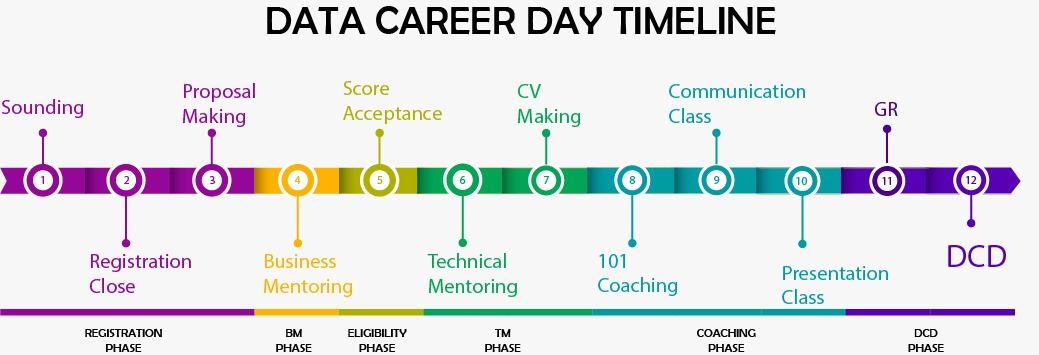
\includegraphics{assets/DCD pace.jpeg}

\hypertarget{pre-requisite-data-career-day}{%
\section{Pre-Requisite Data Career Day}\label{pre-requisite-data-career-day}}

\begin{enumerate}
\def\labelenumi{\arabic{enumi}.}
\tightlist
\item
  \emph{Self-Funding} pada Academy Reguler/Academy Full Stack/Beasiswa Full Stack
\item
  Total score minimal 85\%
\item
  Mengerjakan 5 dari 9 Learn by Building (LBB) (sudah termasuk LBB IP)
\item
  Melakukan pendaftaran saat Registration Pace
\item
  Mengumpulkan proposal project yang akan dikerjakan dalam bentuk link rpubs
\end{enumerate}

\hypertarget{registration}{%
\subsection{Registration}\label{registration}}

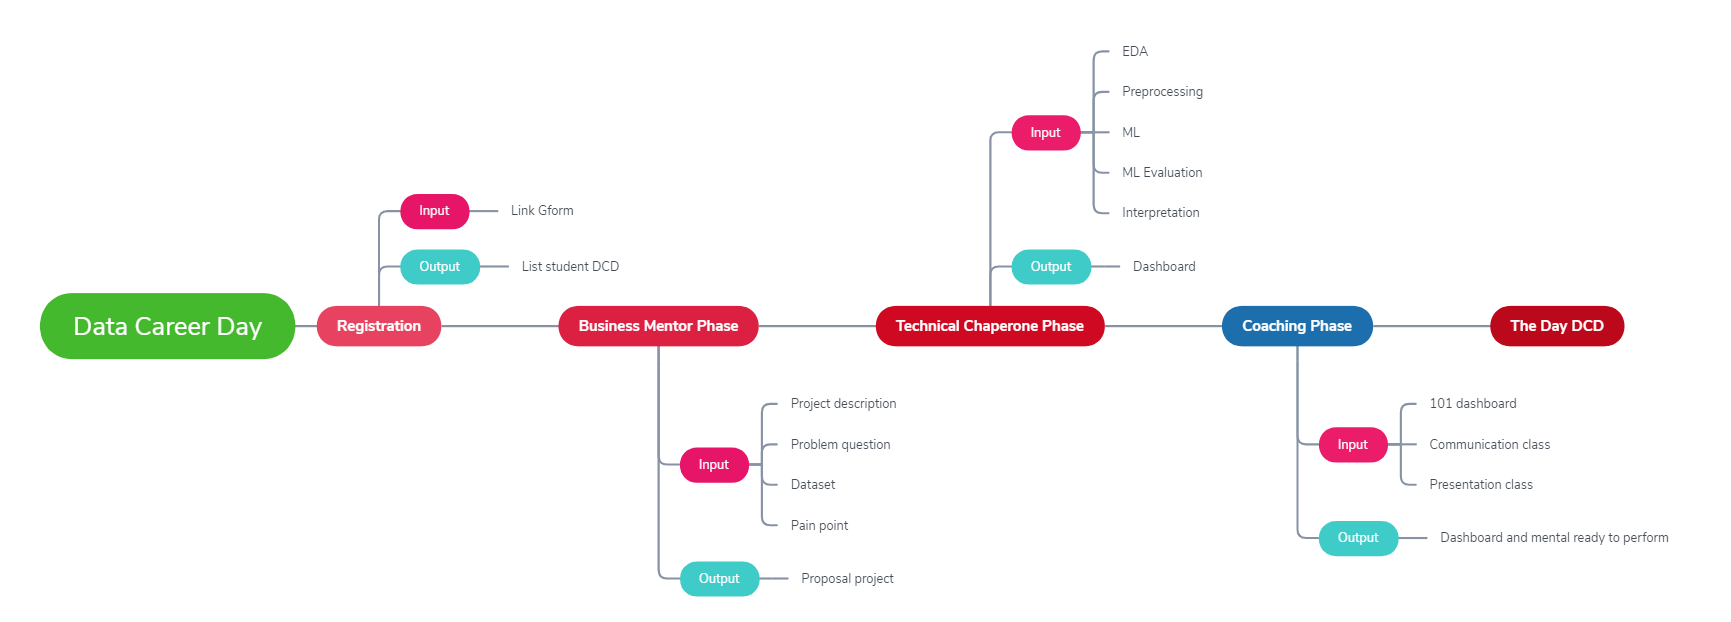
\includegraphics{assets/workflow.png}

\begin{itemize}
\tightlist
\item
  Sebelum Registration
\end{itemize}

\begin{enumerate}
\def\labelenumi{\arabic{enumi}.}
\tightlist
\item
  Hubungi Tata untuk mendapatkan list email student offline yang melakukan pembiayaan sendiri \href{https://docs.google.com/spreadsheets/d/1iZy0AaFASL7IY5BIGZmaOsIqkdX6LR6Mo2gpJZEG2KA/edit\#gid=1637612767}{link}
\item
  Hubungi Tata untuk mendapatkan list email student online yang melakukan pembiayaan sendiri
\item
  Siapkan timeline dari sosialisasi DCD - hari H
\item
  Siapkan slide sosialisasi DCD \href{https://docs.google.com/presentation/d/1acPcUvZG85oEJsLtOGJx3FINGa8Rrhv-CBt-tqAJG_M/edit\#slide=id.p1}{link}
\item
  Sipkan GForm registration (contoh \href{http://bit.ly/registdcd9}{Gform})
\item
  Siapkan publication proposal example \href{http://bit.ly/publicationexample}{link}
\item
  Mendapatkan list Business Mentor (BM) dan Technical Chaperone (TC) (hubungi \textbf{David})
\end{enumerate}

\begin{itemize}
\tightlist
\item
  Selama Registration
\end{itemize}

\begin{enumerate}
\def\labelenumi{\arabic{enumi}.}
\tightlist
\item
  Menyiapkan draft email registrasi DCD \href{https://docs.google.com/document/d/1EDYH3DnzUElPApt2pIBEh9HJV5d7K0OmmsTOs5BmcKI/edit?usp=sharing}{link}
\item
  Mengirimkan email reminder penutupan registration DCD \href{https://docs.google.com/document/d/1EDYH3DnzUElPApt2pIBEh9HJV5d7K0OmmsTOs5BmcKI/edit\#heading=h.yhbqjuew20hg}{link}
\item
  Membuat Gsheet daftar calon peserta DCD (contoh \href{https://docs.google.com/spreadsheets/d/1P_dRfwtu_yTWtPr-RHKjIon_ZXVUdf2RtMXiWMqWrZk/edit?usp=sharing}{Gsheet})
\item
  Melakukan briefing mengenai timeline dan workflow DCD kepada mentor Team (mentoring workflow \href{https://docs.google.com/presentation/d/1iERQj08tN_PHhIKs2RA37kH6IsQ5FzV3uALNC3SsEsk/edit?usp=sharing}{link})
\end{enumerate}

\begin{itemize}
\tightlist
\item
  Setelah Registration
\end{itemize}

\begin{enumerate}
\def\labelenumi{\arabic{enumi}.}
\tightlist
\item
  Melakukan plotting student dengan BM berdasarkan case yang diambil oleh student \href{https://docs.google.com/spreadsheets/d/1P_dRfwtu_yTWtPr-RHKjIon_ZXVUdf2RtMXiWMqWrZk/edit\#gid=1325523908}{link}
\item
  Mengirimkan email mentor assigning kepada calon peserta yang sudah mendaftar (draft email \href{https://docs.google.com/document/d/1EDYH3DnzUElPApt2pIBEh9HJV5d7K0OmmsTOs5BmcKI/edit\#heading=h.bwo0f6c325u7}{mentor assigning})
\item
  Invite student pada channel slack Algoritma Alumni sebagai platform komunikasi
\end{enumerate}

\hypertarget{business-mentor-phase}{%
\subsection{Business Mentor Phase}\label{business-mentor-phase}}

\begin{enumerate}
\def\labelenumi{\arabic{enumi}.}
\tightlist
\item
  Membuat sheet weekly report mentor yang dapat ditransfer untuk mentor pada pace berikutnya \href{https://docs.google.com/spreadsheets/d/1kDS77uA1uYJJyS_Oatv_WJTKEOiYXZgkUyEF3CEXo-M/edit\#gid=223180597}{link}
\item
  Membuat rekapan nilai dan LBB student \href{https://docs.google.com/spreadsheets/d/1kDS77uA1uYJJyS_Oatv_WJTKEOiYXZgkUyEF3CEXo-M/edit\#gid=2041422256}{link}
\item
  Membuat list eligible student dari registration phase, BM phase, TC phase \href{https://docs.google.com/spreadsheets/d/1kDS77uA1uYJJyS_Oatv_WJTKEOiYXZgkUyEF3CEXo-M/edit\#gid=43809870}{link}
\item
  Melakukan follow-up link proposal project student kepada BM dan diletakkan pada satu sheet report mentor
\item
  Plotting student dengan TC
\item
  Mengirimkan reminder pengumpulan terakhir proposal project dan beberapa persyaratan lain (draft email \href{https://docs.google.com/document/d/1EDYH3DnzUElPApt2pIBEh9HJV5d7K0OmmsTOs5BmcKI/edit\#heading=h.eaf8e2km1m0z}{link})
\item
  Mengirimkan email acceptance dan rejected peserta (draft email \href{https://docs.google.com/document/d/1EDYH3DnzUElPApt2pIBEh9HJV5d7K0OmmsTOs5BmcKI/edit\#heading=h.y18cmaj9rlr8}{acceptance BM} \& \href{https://docs.google.com/document/d/1EDYH3DnzUElPApt2pIBEh9HJV5d7K0OmmsTOs5BmcKI/edit\#heading=h.lwhoq5jstbkk}{rejected BM})
\end{enumerate}

\hypertarget{technical-chaperone-phase}{%
\subsection{Technical Chaperone Phase}\label{technical-chaperone-phase}}

\begin{enumerate}
\def\labelenumi{\arabic{enumi}.}
\tightlist
\item
  Monitoring dan follow-up weekly repost progress student kepada TC \href{https://docs.google.com/spreadsheets/d/1kDS77uA1uYJJyS_Oatv_WJTKEOiYXZgkUyEF3CEXo-M/edit\#gid=223180597}{link}
\item
  Mengirimkan email pendataan CV student online saat minggu pertama TC pace \href{http://bit.ly/student-cv-online}{link}
\item
  {[}Optional{]}Request sesi foto ke Kak Mulia dan Ziqka untuk CV student (Hubungi Kak irvan ketersediaan baju graduate student)
\item
  Melakukan pendataan cv student saat minggu terakhir TC pace \href{http://bit.ly/student-cv-dcd9}{link}
\item
  Melakukan rekapitulasi dan cross check \href{http://bit.ly/algo-student-dcd-cv}{informasi CV student DCD} dan \href{http://bit.ly/algo-student-online-cv}{informasi CV student online}
\item
  Pada akhir deadline pengumpulan dan pengisian CV (baik student DCD maupun student online), informasikan kepada Kak Mulia untuk proses pembuatan CV
\item
  Kerjasama marketing mengenai vanue DCD dan teknis hari H DCD
\end{enumerate}

\hypertarget{coaching-phase}{%
\subsection{Coaching Phase}\label{coaching-phase}}

\begin{enumerate}
\def\labelenumi{\arabic{enumi}.}
\tightlist
\item
  Memastikan Veteran yang akan mengisi 101 dashboard, communication class, dan presentation class serta jadwal yang setiap sesi.
\item
  Memastikan setiap peserta hadir dalam setiap sesi.
\item
  Koordinasi dengan marketing untuk GR dan hari-H terkait kesiapan acara
\end{enumerate}

\hypertarget{the-day-dcd}{%
\subsection{The Day DCD}\label{the-day-dcd}}

\begin{enumerate}
\def\labelenumi{\arabic{enumi}.}
\tightlist
\item
  Memastikan student ready saat akan tampil
\item
  Memastikan jalannya acara berjalan dengan lancar dari presentasi student hingga speed dating
\item
  Evaluasi dengan seluruh tim
\end{enumerate}

\hypertarget{piket-guideline}{%
\chapter{Piket Guideline}\label{piket-guideline}}

\hypertarget{tugas-lead-piket}{%
\section{Tugas Lead Piket}\label{tugas-lead-piket}}

\begin{itemize}
\tightlist
\item
  Melakukan pengecekan tiket masuk pada freshdesk.
\item
  Memberikan respon awal tiket yang masuk mengenai eror dan mentoring \textbf{maksimal 2 jam} setelah email diterima pada jam kerja.
\item
  Menugaskan tim piket untuk menjadi PIC Slack Alumni.
\item
  Membuat daftar LBB dan capstone yang masuk dari google classroom.
\item
  Membagi tugas kepada tim piket untuk mengoreksi dan memberikan feedback LBB dan capstone yang telah masuk.
\item
  Lead piket diperkenankan untuk meminta bantuan tim piket membantu menjawab tiket yang masuk pada freshdesk.
\item
  Lead piket yang bertugas dari pagi-sore sebagai instructor ataupun TA dapat meminta bantuan kepada tim piket untuk monitor freshdesk dan classroom.
\end{itemize}

\hypertarget{respon-freshdesk}{%
\section{Respon Freshdesk}\label{respon-freshdesk}}

\begin{itemize}
\tightlist
\item
  Panduan dalam merespon email dengan baik dan benar dapat dilihat pada \href{https://trello-attachments.s3.amazonaws.com/5b178a5917d78094e809e4c9/5f69df1f8aa3e54171468888/de3bd28e0177e532a9de032b35310397/guidelines_(5).html}{dokumentasi berikut}
\item
  Setiap pertanyaan terkait eror, mentoring, dan pertanyaan umum harus diberikan respon awal \textbf{maksimal 2 jam} setelah email diterima pada jam kerja.
\item
  Email atau tiket yang masuk diluar jam kerja akan direspon pada hari berikutnya pada jam kerja.
\end{itemize}

\hypertarget{feedback-learn-by-building-lbb}{%
\section{Feedback Learn by Building (LBB)}\label{feedback-learn-by-building-lbb}}

\begin{itemize}
\tightlist
\item
  LBB yang telah masuk harus diberikan feedback paling lambat \textbf{3 hari} setelah LBB diterima.
\item
  Tim piket yang sedang bertugas \textbf{wajib} mengaktifkan notifikasi google classroom di email.
\item
  Pengumpulan LBB batch yang telah lewat tetap diberikan feedback untuk keperluan Data Career Day (DCD).
\item
  Batch yang telah lewat yang diberikan feedback maksimal 1 batch sebelum batch yang sedang berjalan.
\end{itemize}

\hypertarget{feedback-capstone-project}{%
\section{Feedback Capstone Project}\label{feedback-capstone-project}}

\begin{itemize}
\tightlist
\item
  Capstone project yang telah masuk harus diberikan feedback paling lambat \textbf{2 hari} setelah capstone project diterima.
\item
  Tim piket yang melakukan koreksi dan pemberian feedback capstone project \textbf{wajib langsung memasukkan nilai} pada \href{https://docs.google.com/spreadsheets/d/1cGJ0pn9k9gKCBnceWVwaL9D7BBDMNjLh8uPYlaBlJi8/edit?usp=sharing}{\emph{sheet score}}.
\item
  Tim piket yang melakukan koreksi dan pemberian feedback \textbf{wajib} menyertakan informasi batas waktu perbaikan capstone project kepada student dalam \textbf{waktu 1 minggu} (hari kerja dan hari libur) terhitung sejak capstone project tersebut dikumpulkan.
\item
  Perbaikan capstone project yang dikumpulkan melewati batas waktu yang telah ditetapkan akan tetap diperiksa \textbf{tanpa ada pembaharuan nilai}.
\end{itemize}

\hypertarget{respon-mentoring}{%
\section{Respon Mentoring}\label{respon-mentoring}}

\begin{itemize}
\tightlist
\item
  Dalam periode piket, setiap anggota piket maksimal hanya memberikan sesi mentoring sebanyak 5 sesi. Apabila permintaan mentoring lebih dari itu, maka dianjurkan untuk meminta bantuan tim piket lain atau veteran.
\item
  Permintaan mentoring yang masuk dengan detail mentoring serta jadwal yang sama dapat digabungkan menjadi satu sesi atas persetujuan student yang bersangkutan.
\item
  Dalam 1 sesi mentoring memiliki durasi 1 jam.
\item
  Mentoring yang berhubungan dengan pembahasan capstone project \textbf{tidak akan diproses}.
\item
  Permintaan \textbf{mentoring academy} yang masuk untuk hari Jum'at setiap akhir bulan \textbf{akan dialihkan} untuk hari yang lain.
\item
  Permintaan \textbf{mentoring corporate} yang masuk untuk hari Jum'at setiap akhir bulan \textbf{akan diproses dengan menyesuaikan ketersediaan waktu mentor}.
\end{itemize}

\hypertarget{pelaksanaan-mentoring-offline}{%
\subsection{Pelaksanaan Mentoring Offline}\label{pelaksanaan-mentoring-offline}}

\begin{itemize}
\tightlist
\item
  Protokol tim mentoring offline dapat diakses pada \href{https://docs.google.com/document/d/1L6lA0MJoyhfeYlzFBf-TuuJ8SGhZE4Yc49_kXDWkkLw/edit?usp=sharing}{link berikut}
\item
  Proses mentoring \textbf{hanya} bisa dilakukan pada jam kerja Senin-Jum'at pukul 10:00-18:00.
\item
  Mentoring yang diadakan secara offline dapat ditugaskan kepada mentor yang memiliki akses yang mudah untuk ke kantor.
\item
  Student yang berhalangan hadir dari jadwal mentoring yang telah ditetapkan \textbf{wajib} melakukan konfirmasi melalui email \textbf{\href{mailto:mentor@algorit.ma}{\nolinkurl{mentor@algorit.ma}}} \textbf{maksimal 6 jam} sebelum jadwal mentoring.
\item
  Batas toleransi keterlambatan mentoring sebagai berikut:

  \begin{itemize}
  \tightlist
  \item
    Terlambat \textbf{kurang dari 15 menit} akan tetap diberikan waktu mentoring 1 jam.
  \item
    Terlambat dalam waktu \textbf{15-30 menit} akan diberikan waktu mentoring sesuai jadwal. Contoh mentoring pukul 14:00-15:00, terlambat 30 menit, maka sisa waktu mentoring yaitu 30 menit.
  \item
    Terlambat \textbf{lebih dari 30 menit} dan tanpa konfirmasi akan dianggap telah menggunakan slot mentoring pada minggu tersebut.
  \end{itemize}
\end{itemize}

\hypertarget{pelaksanaan-mentoring-online}{%
\subsection{Pelaksanaan Mentoring Online}\label{pelaksanaan-mentoring-online}}

\begin{itemize}
\tightlist
\item
  Mentoring online akan dilaksanakan melalui platform GMeet.
\item
  Tim mentor akan memberikan undangan mentoring melalui google calendar yang telah berisi informasi detail mentoring.
\item
  Proses mentoring \textbf{hanya} bisa dilakukan pada jam kerja Senin-Jum'at pukul 10:00-18:00.
\item
  Mentoring yang diadakan secara offline dapat ditugaskan kepada mentor yang memiliki akses yang mudah untuk ke kantor.
\item
  Student yang berhalangan hadir dari jadwal mentoring yang telah ditetapkan \textbf{wajib} melakukan konfirmasi melalui email \textbf{\href{mailto:mentor@algorit.ma}{\nolinkurl{mentor@algorit.ma}}} \textbf{maksimal 6 jam} sebelum jadwal mentoring.
\item
  Batas toleransi keterlambatan mentoring sebagai berikut:

  \begin{itemize}
  \tightlist
  \item
    Terlambat \textbf{kurang dari 15 menit} akan tetap diberikan waktu mentoring 1 jam.
  \item
    Terlambat dalam waktu \textbf{15-30 menit} akan diberikan waktu mentoring sesuai jadwal. Contoh mentoring pukul 14:00-15:00, terlambat 30 menit, maka sisa waktu mentoring yaitu 30 menit.
  \item
    Terlambat \textbf{lebih dari 30 menit} dan tanpa konfirmasi akan dianggap telah menggunakan slot mentoring pada minggu tersebut.
  \end{itemize}
\item
  Sertakan template berikut saat memberikan jadwal mentoring online:
\end{itemize}

\begin{quote}
Apabila Anda tidak hadir sesi mentoring lebih dari 30 menit dari jadwal yang telah ditentukan dan tidak memberikan konfirmasi ketidakhadiran sebelum mentoring berlangsung, maka sesi mentoring tersebut dianggap sebagai satu sesi penuh, sehingga slot mentoring berkurang satu untuk minggu tersebut.
\end{quote}

\hypertarget{slack-alumni}{%
\section{Slack Alumni}\label{slack-alumni}}

\begin{itemize}
\tightlist
\item
  Selama periode tim piket, akan dibentuk PIC yang bertugas untuk menjadi moderator dalam channel \texttt{\#r}/\texttt{\#python} pada Slack Alumni.
\item
  PIC ditunjuk oleh lead tim piket selama periode tim piket (2 minggu).
\item
  PIC bertugas memberikan \textbf{update news} dibidang terkait yang bisa memantik untuk berdiskusi dengan alumni
\item
  PIC bertanggung jawab dalam \textbf{menjawab pertanyaan} yang ada di channel Slack Alumni.
\item
  Tim piket yang lain bertugas untuk ikut berpartisipasi dalam diskusi yang ada pada Slack Alumni.
\end{itemize}

\hypertarget{code-style-guide}{%
\chapter{Code Style Guide}\label{code-style-guide}}

\hypertarget{python-code-style-guide}{%
\section{Python Code Style Guide}\label{python-code-style-guide}}

This document is derived from python \href{https://www.python.org/dev/peps/pep-0008/}{pep-8} and \href{https://google.github.io/styleguide/pyguide.html}{google code style guide} and was meant to be used as Algoritma's code standard for python.

\hypertarget{code-layout}{%
\subsection{Code Layout}\label{code-layout}}

\hypertarget{indentation}{%
\subsubsection{Indentation}\label{indentation}}

Use 4 space as indentation. If you have custom code editor, please make sure to set it correctly to prevent indentation inconcistencies. This rule is optional for continuation lines case.

\begin{Shaded}
\begin{Highlighting}[]
\CommentTok{\# Correct }
\ControlFlowTok{if}\NormalTok{ x }\OperatorTok{=} \VariableTok{None}\NormalTok{: }
\NormalTok{    x}\OperatorTok{=}\DecValTok{1} \CommentTok{\# Use 4 space as indentation}

\CommentTok{\# Wrong }
\ControlFlowTok{if}\NormalTok{ x }\OperatorTok{=} \VariableTok{None}\NormalTok{:}
\NormalTok{  x}\OperatorTok{=}\DecValTok{1} \CommentTok{\# Use only 2 space as indentation}

\CommentTok{\# Continuation lines case }
\NormalTok{df }\OperatorTok{=}\NormalTok{ pd.read\_csv(}\StringTok{\textquotesingle{}folder1/folder2/folder3/folder4/such\_a\_long\textbackslash{}}
\StringTok{                 \_ffoldernname/file.csv\textquotesingle{}}\NormalTok{)}
\end{Highlighting}
\end{Shaded}

\hypertarget{blank-lines}{%
\subsubsection{Blank Lines}\label{blank-lines}}

Surround top-level function and class definitions with two blank lines.

Method definitions inside a class are surrounded by a single blank line.

Extra blank lines may be used (sparingly) to separate groups of related functions. Blank lines may be omitted between a bunch of related one-liners (e.g.~a set of dummy implementations).

Use blank lines in functions, sparingly, to indicate logical sections.
In jupyter notebook, you can use new cell in exchange for 2 Blank lines

\begin{Shaded}
\begin{Highlighting}[]
\ImportTok{import}\NormalTok{ re}
\ImportTok{import}\NormalTok{ glob}
\ImportTok{import}\NormalTok{ sys}
\CommentTok{\# Blank line}
\ImportTok{import}\NormalTok{ requests}
\ImportTok{import}\NormalTok{ scrapy}
\CommentTok{\# Blank line}
\ImportTok{from}\NormalTok{ flask }\ImportTok{import}\NormalTok{ Flask}
\ImportTok{from}\NormalTok{ my\_local\_module }\ImportTok{import}\NormalTok{ MyClass}
\CommentTok{\# Blank line}
\CommentTok{\# Blank line}
\KeywordTok{def}\NormalTok{ top\_level\_function1():}
    \ControlFlowTok{pass}
\CommentTok{\# Blank line}
\CommentTok{\# Blank line}
\KeywordTok{def}\NormalTok{ top\_level\_function2():}
    \ControlFlowTok{pass}
\CommentTok{\# Blank line}
\CommentTok{\# Blank line}
\KeywordTok{class}\NormalTok{ TestClass(}\BuiltInTok{object}\NormalTok{):}
    \CommentTok{\# Blank line}
    \KeywordTok{def}\NormalTok{ class\_method1():}
        \ControlFlowTok{pass}
    \CommentTok{\# Blank line}
    \KeywordTok{def}\NormalTok{ class\_method2():}
        \ControlFlowTok{pass}
\CommentTok{\# Blank line}
\CommentTok{\# Blank line}
\KeywordTok{class}\NormalTok{ TestClass2(}\BuiltInTok{object}\NormalTok{):}
    \CommentTok{\# Blank line}
    \KeywordTok{def}\NormalTok{ class2\_method1():}
        \ControlFlowTok{pass}
    \CommentTok{\# Blank line    }
    \KeywordTok{def}\NormalTok{ class2\_method2():}
        \ControlFlowTok{pass}
\end{Highlighting}
\end{Shaded}

\begin{Shaded}
\begin{Highlighting}[]
\CommentTok{\# New logical cell }
\NormalTok{new\_object }\OperatorTok{=}\NormalTok{ MyClass()}
\NormalTok{other\_object }\OperatorTok{=}\NormalTok{ TestClass2(new\_object)}
\end{Highlighting}
\end{Shaded}

\hypertarget{cells}{%
\subsubsection{Cells}\label{cells}}

If some lines of code has different logical plan, you can split it as different cells.

\begin{Shaded}
\begin{Highlighting}[]
\NormalTok{a }\OperatorTok{=}\NormalTok{ read\_something()}
\NormalTok{x1 }\OperatorTok{=}\NormalTok{ doing\_something\_with\_(a)}
\NormalTok{x2 }\OperatorTok{=}\NormalTok{ still\_doing\_something\_with\_a(a)}
\NormalTok{result1 }\OperatorTok{=}\NormalTok{ x1 }\OperatorTok{+}\NormalTok{ x2}
\end{Highlighting}
\end{Shaded}

\begin{Shaded}
\begin{Highlighting}[]
\NormalTok{b }\OperatorTok{=}\NormalTok{ read\_something()}
\NormalTok{y1 }\OperatorTok{=}\NormalTok{ doing\_something\_with\_b(b)}
\NormalTok{y2 }\OperatorTok{=}\NormalTok{ still\_doing\_something\_with\_b(b)}
\NormalTok{result2 }\OperatorTok{=}\NormalTok{ y1 }\OperatorTok{+}\NormalTok{ y2}
\end{Highlighting}
\end{Shaded}

If it belongs to other segments, or if you need some text to explain it, use markdown cells to split it.

\begin{Shaded}
\begin{Highlighting}[]
\NormalTok{plot(result1, result2)}
\end{Highlighting}
\end{Shaded}

\hypertarget{comments}{%
\subsection{Comments}\label{comments}}

Comments that contradict the code are worse than no comments. Always make a priority of keeping the comments up-to-date when the code changes!

Comments should be complete sentences. The first word should be capitalized, unless it is an identifier that begins with a lower case letter (never alter the case of identifiers!).

Block comments generally consist of one or more paragraphs built out of complete sentences, with each sentence ending in a period.

You should use two spaces after a sentence-ending period in multi- sentence comments, except after the final sentence.

Ensure that your comments are clear and easily understandable to other speakers of the language you are writing in.

If you are going to write a fully explained and wide-scoped comment, use markdown cell instead!.

Inline comments should be placed at least 2 space after each code

\begin{Shaded}
\begin{Highlighting}[]
\NormalTok{x }\OperatorTok{=} \DecValTok{2} \OperatorTok{+} \DecValTok{2}  \CommentTok{\# This is a correct inline comment}
\end{Highlighting}
\end{Shaded}

\hypertarget{naming-styles}{%
\subsection{Naming Styles}\label{naming-styles}}

Use \texttt{snake\_style} for naming an object or function

Use \texttt{CamelCaseStyle} for naming a class

Use \texttt{SCREAMING\_SNAKE\_STYLE} for naming a constant object

\begin{Shaded}
\begin{Highlighting}[]
\KeywordTok{class}\NormalTok{ MyOwnClass():}
    \KeywordTok{def} \FunctionTok{\_\_init\_\_}\NormalTok{(}\VariableTok{self}\NormalTok{, api\_key, secret\_key, max\_attempt):}
        \VariableTok{self}\NormalTok{.api\_key }\OperatorTok{=}\NormalTok{ api\_key}
        \VariableTok{self}\NormalTok{.secret\_key }\OperatorTok{=}\NormalTok{ secret\_key}
        \VariableTok{self}\NormalTok{.max\_attempt }\OperatorTok{=}\NormalTok{ max\_attempt}

    \KeywordTok{def}\NormalTok{ send\_message(message):}
        \ControlFlowTok{pass}

\NormalTok{API\_KEY }\OperatorTok{=}\NormalTok{ os.environ([}\StringTok{\textquotesingle{}api\textquotesingle{}}\NormalTok{])}
\NormalTok{SECRET\_KEY }\OperatorTok{=}\NormalTok{ os.environ([}\StringTok{\textquotesingle{}secret\textquotesingle{}}\NormalTok{])}
\NormalTok{MAX\_ATTEMPT }\OperatorTok{=} \DecValTok{3} 

\NormalTok{my\_object }\OperatorTok{=}\NormalTok{ MyOwnClass(API\_KEY, SECRET\_KEY, MAX\_ATTEMPT)}
\end{Highlighting}
\end{Shaded}

\hypertarget{imports}{%
\subsection{Imports}\label{imports}}

Imports should usually be on separate lines:

\begin{Shaded}
\begin{Highlighting}[]
\CommentTok{\# Correct }
\ImportTok{import}\NormalTok{ pandas }
\ImportTok{import}\NormalTok{ numpy }
\end{Highlighting}
\end{Shaded}

\begin{Shaded}
\begin{Highlighting}[]
\CommentTok{\# Wrong }
\ImportTok{import}\NormalTok{ os, re}
\end{Highlighting}
\end{Shaded}

However, using the \texttt{from\ ...\ import\ ...} it's okay to import multiple module / class in one line

\begin{Shaded}
\begin{Highlighting}[]
\CommentTok{\# Correct }
\ImportTok{from}\NormalTok{ tensorflow.keras.layers }\ImportTok{import}\NormalTok{ Dense, Flatten, Conv1D}
\end{Highlighting}
\end{Shaded}

Imports are always put at the top of the file, just after any module comments and docstrings, and before module globals and constants. It should be grouped in the following order:
- Standard library imports.
- Related third party imports.
- Local application/library specific imports.

\begin{Shaded}
\begin{Highlighting}[]
\ImportTok{import}\NormalTok{ os  }\CommentTok{\# Standard library }
\ImportTok{import}\NormalTok{ re }

\ImportTok{import}\NormalTok{ pandas }\ImportTok{as}\NormalTok{ pd  }\CommentTok{\# 3rd party library}
\ImportTok{import}\NormalTok{ tensorflow }\ImportTok{as}\NormalTok{ tf }

\ImportTok{from}\NormalTok{ util }\ImportTok{import}\NormalTok{ tangan\_tuhan }\CommentTok{\# read your own modules}
\end{Highlighting}
\end{Shaded}

Avoid usage of wildcard

\begin{Shaded}
\begin{Highlighting}[]
\CommentTok{\# Not recomended }
\ImportTok{from}\NormalTok{ pandas }\ImportTok{import} \OperatorTok{*}
\end{Highlighting}
\end{Shaded}

\hypertarget{string-quotes}{%
\subsection{String Quotes}\label{string-quotes}}

Prefer single string over double string unless it's needed

\begin{Shaded}
\begin{Highlighting}[]
\CommentTok{\# Correct }
\NormalTok{path }\OperatorTok{=} \StringTok{\textquotesingle{}folder/folder/folder\textquotesingle{}}
\NormalTok{person\_name }\OperatorTok{=} \StringTok{"ya\textquotesingle{}qub"} 
\end{Highlighting}
\end{Shaded}

If you are going to use triple quotes string, always use double string as mentioned in \href{https://www.python.org/dev/peps/pep-0257/}{PEP 257}

\begin{Shaded}
\begin{Highlighting}[]
\CommentTok{\# Correct }
\NormalTok{query }\OperatorTok{=} \StringTok{"""}
\StringTok{        select * }
\StringTok{        from table }
\StringTok{        where }
\StringTok{            age \textgreater{} 10 }
\StringTok{            AND hair is \textquotesingle{}brown\textquotesingle{}}
\StringTok{            AND name like \textquotesingle{}}\SpecialCharTok{\%le}\StringTok{e\%\textquotesingle{}}
\StringTok{        """}
\end{Highlighting}
\end{Shaded}

\hypertarget{whitespaces}{%
\subsection{Whitespaces}\label{whitespaces}}

Always surround these binary operators with a single space on either side: assignment (=), augmented assignment (+=, -= etc.), comparisons (==, \textless, \textgreater, !=, \textless\textgreater, \textless=, \textgreater=, in, not in, is, is not), Booleans (and, or, not).

If operators with different priorities are used, consider adding whitespace around the operators with the lowest priority(ies). Use your own judgment; however, never use more than one space, and always have the same amount of whitespace on both sides of a binary operator:

\begin{Shaded}
\begin{Highlighting}[]
\CommentTok{\# Correct }
\NormalTok{i }\OperatorTok{=}\NormalTok{ i }\OperatorTok{+} \DecValTok{1} 
\NormalTok{y }\OperatorTok{=}\NormalTok{ m}\OperatorTok{*}\NormalTok{x }\OperatorTok{+}\NormalTok{ b}
\NormalTok{y }\OperatorTok{=}\NormalTok{ a }\OperatorTok{+}\NormalTok{ b }\OperatorTok{+}\NormalTok{ c }\OperatorTok{+}\NormalTok{ d}
\NormalTok{y }\OperatorTok{=}\NormalTok{ (a}\OperatorTok{+}\NormalTok{b) }\OperatorTok{+}\NormalTok{ (c}\OperatorTok{/}\NormalTok{d)}
\NormalTok{y }\OperatorTok{=}\NormalTok{ (a}\OperatorTok{*}\NormalTok{b }\OperatorTok{+}\NormalTok{ c) }\OperatorTok{/}\NormalTok{ (f}\OperatorTok{/}\NormalTok{g }\OperatorTok{{-}}\NormalTok{ h)}
\end{Highlighting}
\end{Shaded}

\begin{Shaded}
\begin{Highlighting}[]
\CommentTok{\# Not recomended }
\NormalTok{i }\OperatorTok{=}\NormalTok{ i}\OperatorTok{+}\DecValTok{1}
\NormalTok{y }\OperatorTok{=}\NormalTok{ m}\OperatorTok{*}\NormalTok{x}\OperatorTok{+}\NormalTok{b}
\NormalTok{y }\OperatorTok{=}\NormalTok{ a}\OperatorTok{+}\NormalTok{b}\OperatorTok{+}\NormalTok{c}\OperatorTok{+}\NormalTok{d}
\NormalTok{y }\OperatorTok{=}\NormalTok{ (a}\OperatorTok{+}\NormalTok{b)}\OperatorTok{+}\NormalTok{(c}\OperatorTok{/}\NormalTok{d)}
\NormalTok{y }\OperatorTok{=}\NormalTok{ (a}\OperatorTok{*}\NormalTok{b}\OperatorTok{+}\NormalTok{c)}\OperatorTok{/}\NormalTok{(f}\OperatorTok{/}\NormalTok{g}\OperatorTok{{-}}\NormalTok{h)}
\end{Highlighting}
\end{Shaded}

\hypertarget{other-recomendations}{%
\subsection{Other Recomendations}\label{other-recomendations}}

\hypertarget{dont-repeat-yourself-dry}{%
\subsubsection{Don't Repeat Yourself (DRY)}\label{dont-repeat-yourself-dry}}

Try to avoid repetition in your code!

Consider to create a function if you have reused code. This will create awesome modularity in your code so that you won't waste lots of time debugging.

\begin{Shaded}
\begin{Highlighting}[]
\CommentTok{\# Correct }
\KeywordTok{def}\NormalTok{ measure\_distance(source, target):}
    \ControlFlowTok{return}\NormalTok{ np.linalg.norm(source }\OperatorTok{{-}}\NormalTok{ target)}

\KeywordTok{def}\NormalTok{ some\_function\_a(data):}
\NormalTok{    constant }\OperatorTok{=} \FloatTok{127.4}
\NormalTok{    distance }\OperatorTok{=}\NormalTok{ measure\_distance(constant, data)}
    \ControlFlowTok{return}\NormalTok{ distance}

\KeywordTok{def}\NormalTok{ some\_function\_b(data1, data2):}
\NormalTok{    total }\OperatorTok{=} \DecValTok{0}
    \ControlFlowTok{for}\NormalTok{ i }\KeywordTok{in}\NormalTok{ data1:}
        \ControlFlowTok{for}\NormalTok{ j }\KeywordTok{in}\NormalTok{ data2:}
\NormalTok{            distance }\OperatorTok{=}\NormalTok{ measure\_distance(source, target)}
\NormalTok{            total }\OperatorTok{+=}\NormalTok{ distance}
    \ControlFlowTok{return}\NormalTok{ total}
\end{Highlighting}
\end{Shaded}

\begin{Shaded}
\begin{Highlighting}[]
\CommentTok{\# Wrong }
\KeywordTok{def}\NormalTok{ some\_function\_a(data):}
\NormalTok{    constant }\OperatorTok{=} \FloatTok{127.4}
\NormalTok{    distance }\OperatorTok{=}\NormalTok{ np.linalg.norm(constance }\OperatorTok{{-}}\NormalTok{ data)}
    \ControlFlowTok{return}\NormalTok{ distance}

\KeywordTok{def}\NormalTok{ some\_function\_b(data1, data2):}
\NormalTok{    total }\OperatorTok{=} \DecValTok{0}
    \ControlFlowTok{for}\NormalTok{ i }\KeywordTok{in}\NormalTok{ data1:}
        \ControlFlowTok{for}\NormalTok{ j }\KeywordTok{in}\NormalTok{ data2:}
\NormalTok{            distance }\OperatorTok{=}\NormalTok{ np.linalg.norm(source }\OperatorTok{{-}}\NormalTok{ target)}
\NormalTok{            total }\OperatorTok{+=}\NormalTok{ distance}
    \ControlFlowTok{return}\NormalTok{ total}
\end{Highlighting}
\end{Shaded}

Create a loop over repetitive task

\begin{Shaded}
\begin{Highlighting}[]
\CommentTok{\# Wrong }
\NormalTok{x1 }\OperatorTok{=}\NormalTok{ f(a)}
\NormalTok{x2 }\OperatorTok{=}\NormalTok{ f(b)}
\NormalTok{x3 }\OperatorTok{=}\NormalTok{ f(c)}

\CommentTok{\# Correct }
\NormalTok{x1, x2, x3 }\OperatorTok{=}\NormalTok{ [f(x) }\ControlFlowTok{for}\NormalTok{ x }\KeywordTok{in}\NormalTok{ [a, b, c]]}
\end{Highlighting}
\end{Shaded}


  \bibliography{book.bib,packages.bib}

\end{document}
